\lstinputlisting[language=Matlab]{Cap_4/Es_7/Es_7.m}

La seguente figura mostra il polinomio interpolante le ascisse
di Chebyshev per la funzione di Runge al variare di N grado del polinomio con
$N=2,4,6,8...40$
\\
\begin{figure}[H]
  \label{Cap_4_Es_7(2)}
  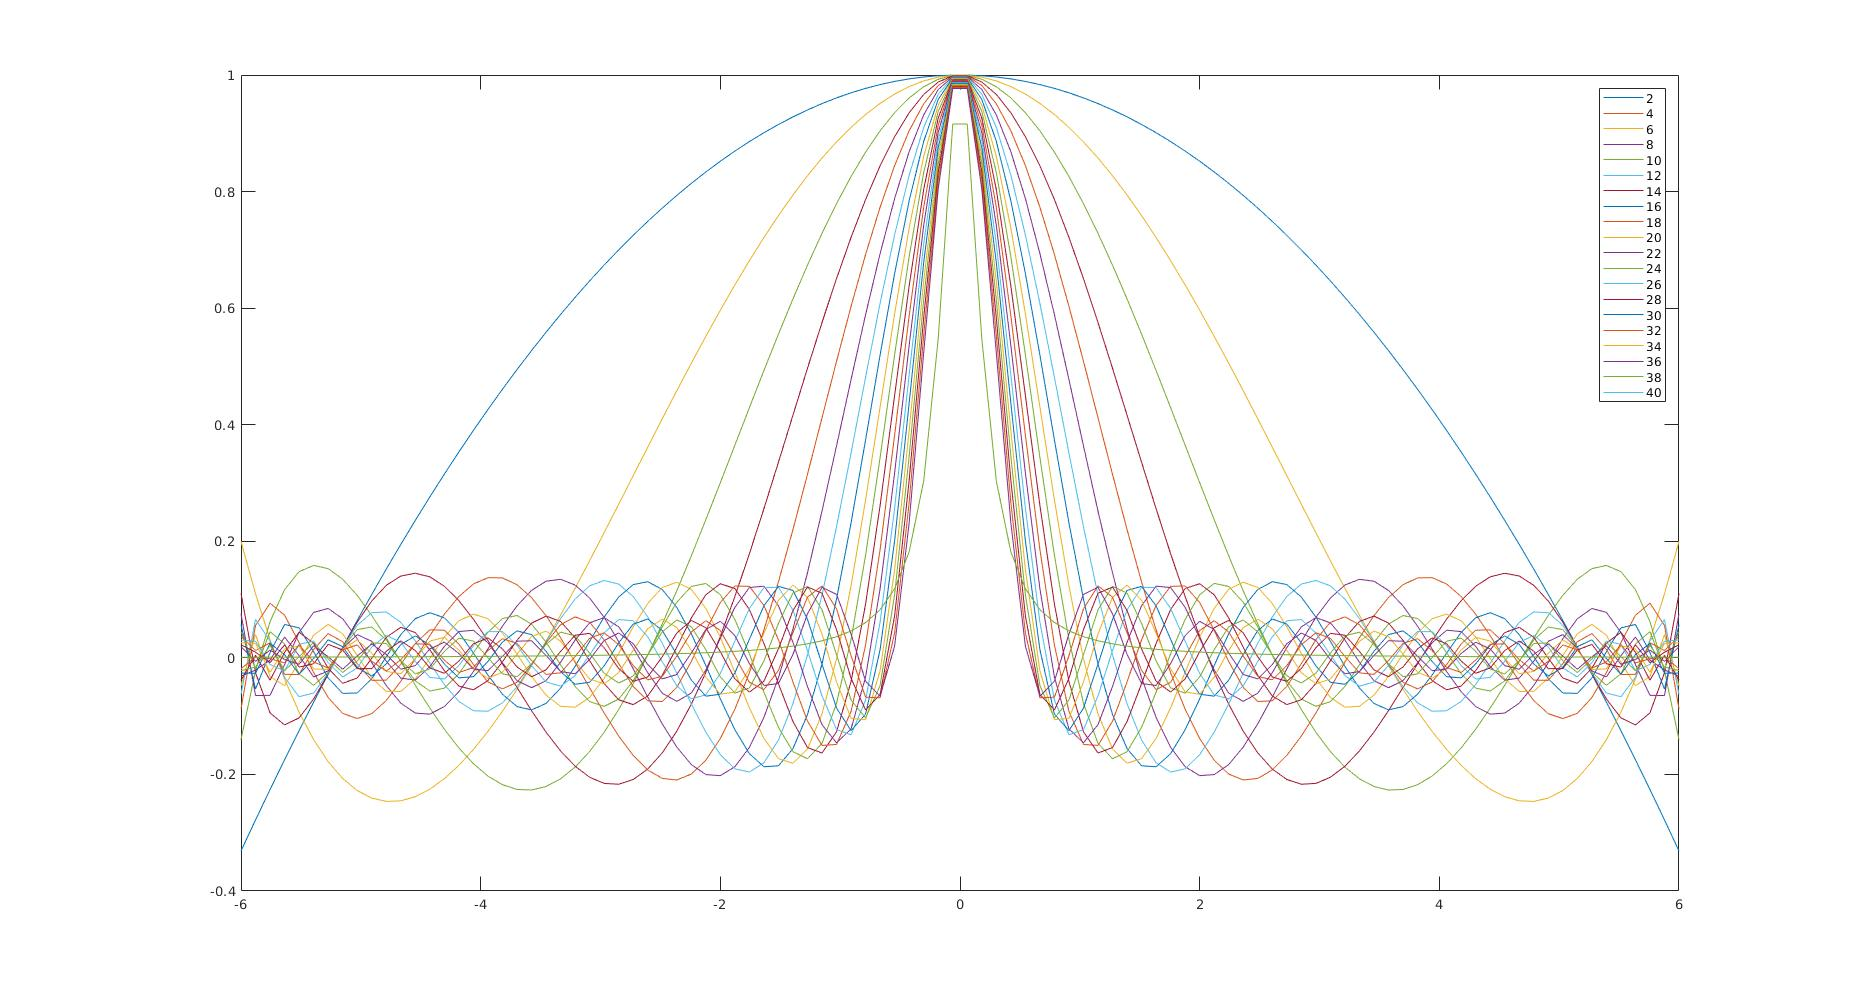
\includegraphics[left, width=130px]{Plot/Cap_4_Es_7(2)}
    \caption{Polinomio di Lagrange al variare di N}
\end{figure}
La seguente tabella mostra invece la stima dell'errore al variare di N (grado del polinomio interpolante) tramite la norma euclidea 
della differenza tra le fi della funzione di Ruge e quelle del polinomio di Lagrange.

\begin{center}
	\begin{tabular}{|c|c|}
		\hline
			N & $|(f(x)-y|$ \\
    \hline
    $2$  & $65.1749$ \\
    $4$  & $51.8929$ \\
    $6$  & $44.2988$ \\
    $8$  & $39.3066$ \\
    $10$ & $35.6975$ \\
    $12$ & $32.9190$ \\
    $14$ & $30.7265$ \\
    $16$ & $28.8977$ \\
    $18$ & $27.3972$ \\
    $20$ & $26.0781$ \\
    $22$ & $24.9797$ \\
    $24$ & $23.9751$ \\
    $26$ & $23.1381$ \\
    $28$ & $22.3469$ \\
    $30$ & $21.6900$ \\
    $32$ & $21.0518$ \\
    $34$ & $20.5221$ \\
    $36$ & $20.0008$ \\
    $38$ & $19.5675$ \\
    $40$ & $19.1448$ \\
		\hline
	\end{tabular}
\end{center} 